\documentclass[a4paper,10pt,bg=print]{dndbook} %a4, 10pt, bg=print / full
\usepackage[english]{babel} %language
\usepackage[utf8]{inputenc} %lovely utf-8
\usepackage{graphicx} %images
\usepackage{array} %allways use this shit, idk why
\usepackage{tikz} %draw stuff
\usepackage{ifthen} %draw stuff
\usetikzlibrary{calc,fadings} %draw stuff
\usepackage{xspace} %usefull idk, allways import this stuff
\usepackage{setspace} %don't ask, kind of like it...
\usepackage{pgfplots}
\usepackage{tabularx} % table
\usepackage[singlelinecheck=false]{caption} %idk dndbook...
\usepackage{listings} %idk dndbook...
\usepackage{stfloats} %idk dndbook
\usepackage{yfonts}
\usepackage{aurical}
\usepackage[T1]{fontenc}

\graphicspath{ {./images/} }

\pagestyle{empty} % no footer

\geometry { % paper type + spacing
	a4paper,
	top=2cm,
	bottom=2cm,
	left=2cm,
	right=2cm
}
\newcommand*\circled[2][2pt]{
	\tikz
	[
		decoration={
			random steps,
			amplitude=1pt,
			segment length=5pt
		},
		baseline=(char.base)
	]{
		\node
		[
			decorate,
			shape=circle,
			draw,
			inner sep=#1-1pt
		]
		(char) {#2};
	}
}

\singlespacing
\makeatletter

\def \license {GNU Free Documentation License (https://www.gnu.org/licenses/fdl-1.3)}
\def \author {Sven Hugi}%if you edit this document, add your name... <3

%highlighting with some random effect -> looks handmade and i love it... you can use this in you texts
\newcommand\hl[2][yellow]{
	\begin{tikzpicture}[
	baseline,
	decoration={random steps,amplitude=1pt,segment length=15pt},
	outer sep=-15pt, inner sep = 0pt
	]
	\node[decorate,rectangle,fill=#1,anchor=text]{#2\xspace};
	\end{tikzpicture}
}
% colors:

% bgtan
% bgtan2018
% pagegold

% titlered
% titlegold
% rulered
% contourgray

% BrGreen
% PhbLightGreen
% PhbLightCyan
% PhbMauve
% PhbTan
% DmgLavender
% DmgCoral
% DmgSlateGray
% DmgLilac

%config:
\def\Name{Seirilia}
\def\offset{-5.67} % change, if the line at the top is staggered -> -5.67 is the default value -> should work in ~100% of the cases

\def\CharaClass{Warlock}
\def\Level{1}
\def\Background{Entertainer}
\def\Playername{}
\def\Race{Tiefling}
\def\Alignment{Neutral Good}
\def\EP{} % not set

\def\Speed{30}
\def\Initiative{+2}
\def\AC{13}
\def\Prof{+2}

\def\MaxHP{9}
\def\HitDice{d8}

\def\Str{7}
\def\Dex{15}
\def\Con{12}
\def\Int{14}
\def\Wis{11}
\def\Cha{20}

\def\StrMod{-2}
\def\DexMod{+2}
\def\ConMod{+1}
\def\IntMod{+2}
\def\WisMod{0}
\def\ChaMod{+5}

\def\StrSave{-2}
\def\DexSave{+2}
\def\ConSave{+1}
\def\IntSave{+2}
\def\WisSave{+2}
\def\ChaSave{+7}

% save profs
\def\firstStat{Cha}
\def\secondStat{Wis}

% modifiers for skills (add prof bonus if prof)
%str
\def\Athletics{-2}
%dex
\def\Acrobatics{+4}
\def\SleightOfHand{+2}
\def\Stealth{+2}
%int
\def\Arcana{+4}
\def\History{+2}
\def\Investigation{+2}
\def\Nature{+2}
\def\Religion{+2}
%wis
\def\AnimalHandling{0}
\def\Insight{0}
\def\Medicine{0}
\def\Perception{0}
\def\Survival{0}
%cha
\def\Deception{+7}
\def\Intimidation{+5}
\def\Performance{+7}
\def\Persuasion{+5}

% prof (0/1)
\def\AthleticsProf{0}
%dex
\def\AcrobaticsProf{1}
\def\SleightOfHandProf{0}
\def\StealthProf{0}
%int
\def\ArcanaProf{1}
\def\HistoryProf{0}
\def\InvestigationProf{0}
\def\NatureProf{0}
\def\ReligionProf{0}
%wis
\def\AnimalHandlingProf{0}
\def\InsightProf{0}
\def\MedicineProf{0}
\def\PerceptionProf{0}
\def\SurvivalProf{0}
%cha
\def\DeceptionProf{1}
\def\IntimidationProf{0}
\def\PerformanceProf{1}
\def\PersuasionProf{0}

\def\Age{16}
\def\Height{5'5}
\def\Weight{90 lb}
\def\Skin{purple}
\def\Eyes{green}
\def\Hair{Short grey}

\def\SpellAbility{Cha}
\def\SpellAtk{+7}
\def\SpellSaveDC{15}

\def\FirstLevelSlots{1}
\def\SecondLevelSlots{0}
\def\ThirdLevelSlots{0}
\def\FourthLevelSlots{0}
\def\FifthLevelSlots{0}
\def\SixthLevelSlots{0}
\def\SeventhLevelSlots{0}
\def\EightLevelSlots{0}
\def\NinthLevelSlots{0}

\def\Cantrips{
	\small %uncomment for non-wizards...
	\begin{tabularx}{\linewidth}{lX}
		\textbf{Mage Hand} & 1 Action, 30ft, 1 Min, Can’t attack, activate magical items, or carry more than 10 pounds. V, S\\
		\textbf{Eldritch Blast} & 1 Action, 120ft, 1d10 force damage, V, S\\
		\textbf{Thaumaturgy} & 1 Action, 30ft, 1 Min, max 3 at the time, Effects: 1) Your voice booms up to three times as loud 2) flames flicker, brighten, dim, or change color 3) harmless tremors in the ground  4) instantaneous sound that originates from a point of your choice 5) instantaneously fly open or slam shut an unlocked door or window 6) alter the appearance of your eyes. V\\
		\textbf{Light} & 1 Action, Touch, 1h, Dex-save, 10ft x 10ft x 10ft, the object sheds bright light in a 20-foot radius and dim light for 20 feet. V, M (a firefly or phosphorescent moss)\\
		\textbf{Sacred Flame} & 1 Action, 60ft, 1d8 radiant damage, 1 target, Dex-save, no benefit from cover. V, S\\
	\end{tabularx}
}
\def\FirstLevelSpells{
	\begin{tabularx}{\linewidth}{lX}
		\textbf{Cure Wounds} & 1 Action, A creature you touch regains 1d8 + your spellcasting ability modifier of hit points. This spell has no effect on undead or constructs. V, S\\
	\end{tabularx}
}
% you will not be able to just add spells of 2nd lvl and higher, but you can use my template, if you want to level up with this character

% todo
\def\Description{
	
}

\def\WeaponEquipment{
	%max 4 weapons -> with some only 3, with morningstar & co 5
		\textbf{4 Daggers}\\
		\raggedleft
		+4 1d4 + 2 Piercing\\
		Light, Finesse, Thrown (20/60)\\
		\raggedright
}

\def\WeaponProf{
	%warning, empty itemize throws error -> empty item placed -> don't let this unused...
	\begin{itemize}
		\item Simple weapons
	\end{itemize}
}
\def\ArmorProf{
	\begin{itemize}
		\item Light Armor
	\end{itemize}
}
\def\LanguageProf{
	\begin{itemize}
		\item Common
		\item Infernal
	\end{itemize}
}
\def\ToolProf{
	\begin{itemize}
		\item Disguise kit
		\item Flute
	\end{itemize}
}

\def\ClassFeature{
	\begin{tabularx}{\textwidth}{lX}
		\textbf{Pact Magic}	& Regain Spellslots form a short rest. You can use an arcane focus as a spellcasting focus for your warlock spells.\\
	\end{tabularx}
	\textcolor{titlered}{\large The Celestial}\\
	\begin{tabularx}{\textwidth}{lX}
		\textbf{Healing Light} & You have a pool of 1 + your warlock level d6s per long rest. As a bonus action, you can heal one creature you can see within 60 feet of you, spending dice from the pool. The maximum number of dice you can spend at once equals your Charisma modifier.\\
	\end{tabularx}
}
\def\RaceFeature{
	\begin{tabularx}{\textwidth}{lX}
		\textbf{Darkvision}	& You can see in dim light within 60 feet of you as if it were bright light, and in darkness as if it were dim light. You can’t discern color in darkness.\\
		\textbf{Hellish Resistance.} & Resistance to fire damage.\\
		\textbf{Infernal Legacy.} & You know the Thaumaturgy cantrip, charisma is your spellcasting ability.
	\end{tabularx}
}
\def\BackgroundFeature{
	\begin{tabularx}{\textwidth}{lX}
		\textbf{By Popular Demand}	& You can always find a place to perform. At such a place, you receive free lodging and food, as long as you perform each night\\
	\end{tabularx}
}

%static -> don't use for changing stuff, like arows, food etc
% gold from background: 15
\def\Equipment{
	\begin{tabularx}{\textwidth}{lX}
		\textbf{Flute}&\\
		\textbf{Costume}&\\
		\textbf{Favor of an admirer} & love letter\\
		\textbf{Backpack}&\\
		\textbf{Crowbar}&\\
		\textbf{Hammer}&\\
		\textbf{Pitons}& 10\\
		\textbf{Torches}& 10\\
		\textbf{Tinderbox}&\\
		\textbf{Rations}& 10 days\\
		\textbf{Waterskin}&\\
		\textbf{Rope}& 50ft\\
		\textbf{component pouch}&\\
		\textbf{Leather armor} & AC 11 + dex
		
	\end{tabularx}
}

%%%%%%%%%%%%%%%%%%%%%%%%%%%%%%%%%Document%%%%%%%%%%%%%%%%%%%%%%%%%%%%%%%%%
\begin{document}
	\begin{minipage}[t]{.5\linewidth} % head left
		\begin{tabularx}{\textwidth}{XXX}
			\multicolumn{3}{X}{\Fontauri\Name}\\\hline
			\multicolumn{3}{X}{\tiny{Character Name}}\\
			\AC & \Initiative & \Speed {\small$^{ft}$}\\\hline
			\tiny{AC}&\tiny{Initiative}&\tiny{Speed}\\
			\HitDice&\Level&\\\hline
			\tiny{Hit Dice}&\tiny{Total}&\tiny{Used}\\
			\MaxHP&&\\\hline
			\tiny{Max Hp}&\tiny{Hp}&\tiny{Temp Hp}\\
			\Prof&&\\\hline
			\tiny{Proficiency Bonus}
		\end{tabularx}
	\end{minipage}%
	\begin{minipage}[t]{.5\linewidth} % head right
		\strut\vspace*{\offset\baselineskip}\newline %correct offset because of a fontsize and b minipage
		\begin{tabularx}{\textwidth}{XXX}
			\CharaClass\space\Level &\Background &\Playername\\\hline
			\tiny{Class \& Level}	& \tiny{Background}	&\tiny{Player Name}\\
			\Race &\Alignment &\EP\\\hline
			\tiny{Race}	& \tiny{Alignment}	&\tiny{EP}\\
		\end{tabularx}\vspace*{.125cm}\\
		\Fontauri\large{
			\begin{tabularx}{\linewidth}{XXXXXX}
				Str & Dex & Con & Int & Wis & Cha \\ \hline
				\Str & \Dex & \Con & \Int & \Wis & \Cha\\
				\ifthenelse{\equal{\firstStat}{Str}}{$\bullet$}{\ifthenelse{\equal{\secondStat}{Str}}{$\bullet$}{}} &
				\ifthenelse{\equal{\firstStat}{Dex}}{$\bullet$}{\ifthenelse{\equal{\secondStat}{Dex}}{$\bullet$}{}} &
				\ifthenelse{\equal{\firstStat}{Con}}{$\bullet$}{\ifthenelse{\equal{\secondStat}{Con}}{$\bullet$}{}} &
				\ifthenelse{\equal{\firstStat}{Int}}{$\bullet$}{\ifthenelse{\equal{\secondStat}{Int}}{$\bullet$}{}} &
				\ifthenelse{\equal{\firstStat}{Wis}}{$\bullet$}{\ifthenelse{\equal{\secondStat}{Wis}}{$\bullet$}{}} &
				\ifthenelse{\equal{\firstStat}{Cha}}{$\bullet$}{\ifthenelse{\equal{\secondStat}{Cha}}{$\bullet$}{}}\\
				\StrMod & \DexMod & \ConMod & \IntMod & \WisMod & \ChaMod\\
				\StrSave & \DexSave & \ConSave & \IntSave & \WisSave & \ChaSave
			\end{tabularx}
	}
	\end{minipage}\vspace*{.25cm}\\
	\begin{minipage}[t]{.25\linewidth}\normalsize
		{\LARGE Skills}\\
		\textcolor{titlered}{\large Strength \StrMod \ifthenelse{\equal{\firstStat}{Str}}{$\bullet$}{\ifthenelse{\equal{\secondStat}{Str}}{$\bullet$}{}}}\\
		\begin{tabularx}{\textwidth}{lXr}
			\ifthenelse{\equal{\AthleticsProf}{1}}{$\bullet$}{}&Athletics&\Athletics\\
		\end{tabularx}
		\textcolor{titlered}{\large Constitution \ConMod \ifthenelse{\equal{\firstStat}{Con}}{$\bullet$}{\ifthenelse{\equal{\secondStat}{Con}}{$\bullet$}{}}}\\
		\textcolor{titlered}{\large Dexterity \DexMod \ifthenelse{\equal{\firstStat}{Dex}}{$\bullet$}{\ifthenelse{\equal{\secondStat}{Dex}}{$\bullet$}{}}}\\
		\begin{tabularx}{\textwidth}{lXr}
			\ifthenelse{\equal{\AcrobaticsProf}{1}}{$\bullet$}{}&Acrobatics&\Acrobatics\\
			\ifthenelse{\equal{\SleightOfHandProf}{1}}{$\bullet$}{}&Sleight of Hand&\SleightOfHand\\
			\ifthenelse{\equal{\StealthProf}{1}}{$\bullet$}{}&Stealth&\Stealth\\
		\end{tabularx}
		\textcolor{titlered}{\large Intelligence \IntMod \ifthenelse{\equal{\firstStat}{Int}}{$\bullet$}{\ifthenelse{\equal{\secondStat}{Int}}{$\bullet$}{}}}\\
		\begin{tabularx}{\textwidth}{lXr}
			\ifthenelse{\equal{\ArcanaProf}{1}}{$\bullet$}{}&Arcana&\Arcana\\
			\ifthenelse{\equal{\HistoryProf}{1}}{$\bullet$}{}&History&\History\\
			\ifthenelse{\equal{\InvestigationProf}{1}}{$\bullet$}{}&Investigation&\Investigation\\
			\ifthenelse{\equal{\NatureProf}{1}}{$\bullet$}{}&Nature&\Nature\\
			\ifthenelse{\equal{\ReligionProf}{1}}{$\bullet$}{}&Religion&\Religion\\
		\end{tabularx}
		\textcolor{titlered}{\large Wisdom \WisMod \ifthenelse{\equal{\firstStat}{Wis}}{$\bullet$}{\ifthenelse{\equal{\secondStat}{Wis}}{$\bullet$}{}}}\\
		\begin{tabularx}{\textwidth}{lXr}
			\ifthenelse{\equal{\AnimalHandlingProf}{1}}{$\bullet$}{}&Animal Handling&\AnimalHandling\\
			\ifthenelse{\equal{\InsightProf}{1}}{$\bullet$}{}&Insight&\Insight\\
			\ifthenelse{\equal{\MedicineProf}{1}}{$\bullet$}{}&Medicine&\Medicine\\
			\ifthenelse{\equal{\PersuasionProf}{1}}{$\bullet$}{}&Perception&\Perception\\
			\ifthenelse{\equal{\SurvivalProf}{1}}{$\bullet$}{}&Survival&\Survival\\
		\end{tabularx}
		\textcolor{titlered}{\large Charisma \ChaMod \ifthenelse{\equal{\firstStat}{Cha}}{$\bullet$}{\ifthenelse{\equal{\secondStat}{Cha}}{$\bullet$}{}}}\\
		\begin{tabularx}{\textwidth}{lXr}
    		\ifthenelse{\equal{\DeceptionProf}{1}}{$\bullet$}{}&Deception&\Deception\\
			\ifthenelse{\equal{\IntimidationProf}{1}}{$\bullet$}{}&Intimidation&\Intimidation\\
			\ifthenelse{\equal{\PerformanceProf}{1}}{$\bullet$}{}&Performance&\Performance\\
			\ifthenelse{\equal{\PersuasionProf}{1}}{$\bullet$}{}&Persuasion&\Persuasion\\
		\end{tabularx}
		\textcolor{titlered}{\large Weapons}\linebreak
		\WeaponEquipment
	\end{minipage}%
	\begin{minipage}[t]{.25\linewidth}\normalsize
		{\LARGE Proficiencies}
		\textcolor{titlered}{\large Weapons}\\
		\WeaponProf
		\textcolor{titlered}{\large Armor}\\
		\ArmorProf
		\textcolor{titlered}{\large Language}\\
		\LanguageProf
		\textcolor{titlered}{\large Tools}\\
		\ToolProf
	\end{minipage}%
	\begin{minipage}[t]{.5\linewidth}\raggedleft\normalsize
		{\LARGE Features}\\
		\textcolor{titlered}{\large \Background}\\
		\BackgroundFeature
		\textcolor{titlered}{\large \Race}\\
		\RaceFeature
		\textcolor{titlered}{\large \CharaClass}\\
		\ClassFeature
	\end{minipage}\\
	\begin{minipage}[t][\textheight]{.5\linewidth}\normalsize
		{\LARGE Equipment}\\
		\Equipment
	\end{minipage}%
	\begin{minipage}[t][\textheight]{.5\linewidth}\normalsize
		\begin{tabularx}{\textwidth}{XXX}
			&&\\\hline
			\tiny{PP}&\tiny{GP}	&\tiny{EP}\\
			&&\\\hline
			\tiny{SP}& \tiny{CP}&
		\end{tabularx}\vspace*{.25cm}\\
		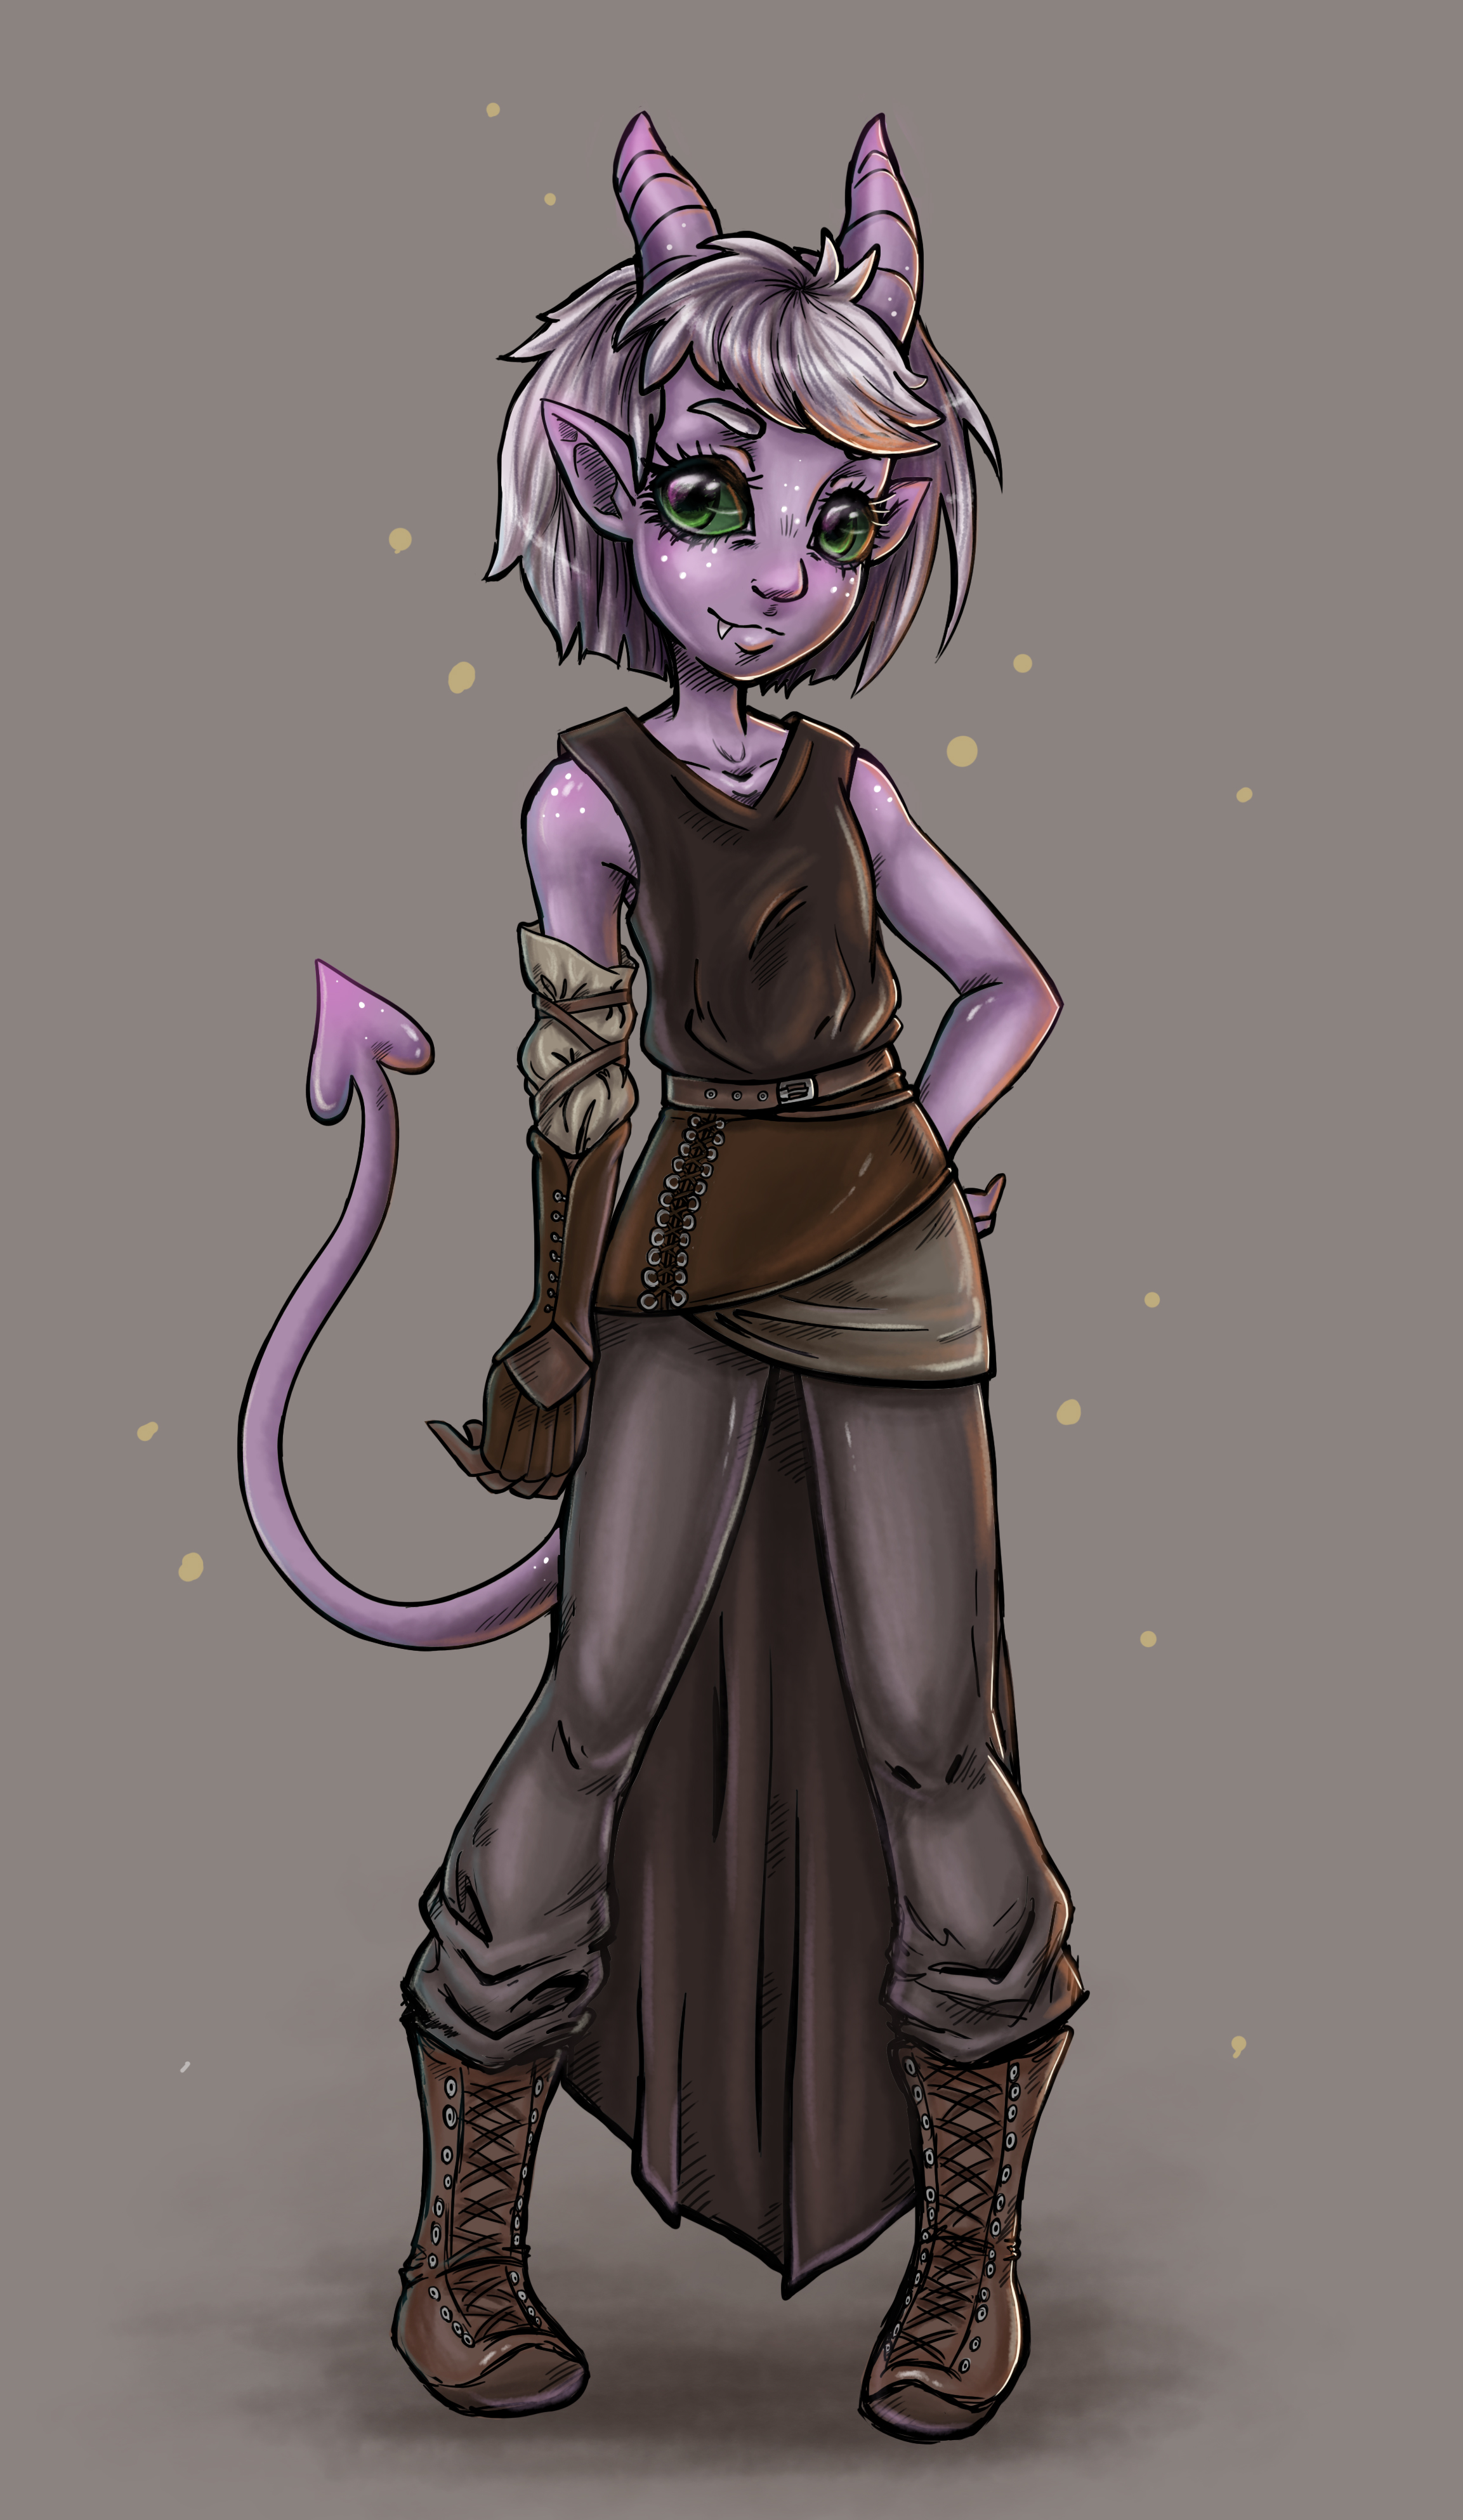
\includegraphics[width=\linewidth]{Character.png}\vspace*{.25cm}\\
		\begin{tabularx}{\textwidth}{XXX}
			\Age &\Height &\Weight\\\hline
			\tiny{Age}	& \tiny{Height}	&\tiny{Weight}\\
			\Eyes &\Skin &\Hair\\\hline
			\tiny{Eyes}	& \tiny{Skin}	&\tiny{Hair}\\
		\end{tabularx}
		{\LARGE Character Description}\\
		{\scriptsize\Description}
	\end{minipage} %
	{\huge Spellcasting}
	\begin{center}\normalsize
		\begin{tabularx}{\textwidth}{XXX}
			\SpellAbility &\SpellAtk &\SpellSaveDC\\\hline
			\tiny{Spellcasting Ability}	& \tiny{Spell Attack Bonus}	&\tiny{Spell Save DC}
		\end{tabularx}
		\begin{tabularx}{\linewidth}{XXXXXXXXX}
			1&2&3&4&5&6&7&8&9\\\hline
			\FirstLevelSlots&
			\SecondLevelSlots&
			\ThirdLevelSlots&
			\FourthLevelSlots&
			\FifthLevelSlots&
			\SixthLevelSlots&
			\SeventhLevelSlots&
			\EightLevelSlots&
			\NinthLevelSlots
		\end{tabularx}
	\end{center}
	\begin{minipage}[t]{1\linewidth}\scriptsize
		\textcolor{titlered}{\large Cantrips}\\
		\Cantrips
		\textcolor{titlered}{\large 1st Level}\\
		\FirstLevelSpells
	\end{minipage}%
\end{document}